\lhead{\textbf{Basic Algorithms, Fall 2024 \\ CSCI-UA.0310-001}}
\chead{\Large{\textbf{Homework 1}}}
\rhead{\textbf{Instructor: Rotem Oshman \\ Name: Ishan Pranav}}
\runningheadrule
\firstpageheadrule
\cfoot{}
\subsection*{References}
No collaborators or outside sources were referenced.
\subsection*{Question 1}
Prove the following equality using induction on $n$:\footnote{Recall that $\mathbb{N}$ denotes the set $\{1,2,\ldots\}$.}
    \begin{align}
    (1-r)(1+r+r^2+ \cdots +r^{n-1}) = 1-r^n \text{ for all } n \in \mathbb{N}\;. \label{eq:geometric-sum}
    \end{align}
\begin{enumerate}
    \item Check the base case ($n=1$).
\begin{solution}
\textit{Basis. }Consider $n=1$. Note $(1-r)(r^{1-1})=(1-r)=(1-r^1)$. Therefore $(1-r)(1+r+r^2+\cdots+r^{n-1})=1-r^n$ for $n=1$.
\end{solution}   
    \item Prove the inductive step.
\begin{solution}
\textit{Hypothesis. }Let $k\in\mathbb{N}$. Of course, $k\geq 1$. Consider $n=k$. Assume the result is true for $n=k$; that is, assume $(1-r)(1+r+r^2+\cdots+r^{k-1})=1-r^k$.\\

\textit{Inductive step. }Consider $n=k+1$. By the inductive hypothesis, $(1-r)(1+r+r^2+\cdots+r^{k-1})=1-r^k$. Observe
\begin{align*}
(1-r)(1+r+r^2+\cdots+r^{k-1})&=1-r^k\\
(1-r)r^k+(1-r)(1+r+r^2+\cdots+r^{k-1})&=1-r^k+(1-r)r^k\\
(1-r)(1+r+r^2+\cdots+r^{(k+1)-1})&=1-r^k+r^k-r^{k+1}\\
&=1-r^{k+1}.
\end{align*}
Hence, by the principle of mathematical induction, for all $n\in\mathbb{N}$, we have $(1-r)(1+r+r^2+\cdots+r^{n-1})=1-r^n$.$~\square$
\end{solution}
    \item Using Eq.~\eqref{eq:geometric-sum}, evaluate the following sum:
    \begin{align*}
        \sum_{i = 0}^n 2^i \cdot 3^{n-i}
        =
        3^n + 2\cdot 3^{n-1} + 2^2 \cdot 3^{n-2} + \cdots + 2^n =\; ???\;
    \end{align*}
\begin{solution}
Observe
\begin{align*}
\sum_{i=0}^{n}{2^i\cdot3^{n-i}}&=3^n\sum_{i=0}^{n}{2^i\cdot3^{-i}}\\
&=3^n\sum_{i=0}^n{\left(\frac{2}{3}\right)^i}\\
&=3^n\left[1+\frac{2}{3}+\left(\frac{2}{3}\right)^2+\cdots+\left(\frac{2}{3}\right)^{(n+1)-1}\right]\\
&=3^n\left[\frac{\left(1+\frac{2}{3}+\left(\frac{2}{3}\right)^2+\cdots+\left(\frac{2}{3}\right)^{(n+1)-1}\right)\left(1-\frac{2}{3}\right)}{1-\frac{2}{3}}\right].
\end{align*}
Using the result from Eq.~\eqref{eq:geometric-sum}, we have
\begin{align*}
\sum_{i=0}^{n}{2^i\cdot3^{n-i}}&=3^n\left[\frac{1-\left(\frac{2}{3}\right)^{n+1}}{1-\frac{2}{3}}\right]\\
&=3^{n+1}\left[1-\left(\frac{2}{3}\right)^{n+1}\right]\\
&=3^{n+1}-2^{n+1}.
\end{align*}
Thus $\sum_{i=0}^{n}{2^i\cdot3^{n-i}}=3^{n+1}-2^{n+1}$.$~\square$
\end{solution}
\end{enumerate}
\newpage
\subsection*{Question 2}
Find a flaw in the following ``proof by induction'' (see Figure~\ref{fig:horse} for an illustration). In particular, state why the inductive step is incorrect:
\vspace{0.5cm}
\noindent \textbf{Claim:} For all $n \in \mathbb{N}$, and any set of $n$ horses, all horses in the set have the same color.
\begin{enumerate}
    \item Base Case ($n=1$): If there is just one horse in the set, obviously all horses have the same color.
    \item Inductive Step: Suppose the induction hypothesis holds for all $1,2,\ldots,n$. Our goal is to prove the statement for sets of $n+1$ horses. So take any such set. Now exclude one horse, call this horse $A$, and look at the set of $n$ remaining horses. By the induction hypothesis, they all have the same color. Now exclude a different horse, call it $B$, and look at the set of $n$ remaining horses, which includes horse $A$. Then, all horses in this set must also have the same color. This implies that $A$ and $B$ also have the same color. Hence, we obtain that all $n+1$ horses in our set have the same color, ``proving'' the claim. 
\end{enumerate}
\begin{solution}
The error is in the inductive step. First, the author takes a set of $n+1$. The author must show that all horses in this set have the same color. To do this, the author removes horse $A$. By the strong induction hypothesis, the remaining $n$ horses have the same color. To complete the proof, the author's objective is to show that $A$ has the same color as the remaining $n$ horses.\\

Then, the author removes another horse $B$ where $B\neq A$ and groups the other $n$ horses, including $A$. This is an error because it presumes that the induction hypothesis applies to a group of $n$ horses which includes $A$, even though that fact remains unproven.
\end{solution}
\begin{figure}[h]
    \centering
    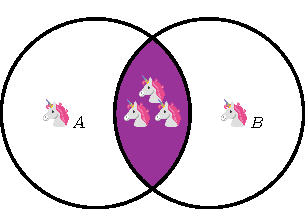
\includegraphics{../images/horse_venn.pdf}
    \caption{Horses $A$ and $B$, with all the rest of the horses lying in the violet region common to both sets.}
    \label{fig:horse}
\end{figure}
\newpage
\subsection*{Question 3}
Recall the {\sc Insertion-Sort} algorithm discussed in the lecture:
\begin{code}
	{\sc Insertion-Sort}$(A,n)$\\
	1. \> \For $j=2$ \To $n$\\
	2. \> \> $key=A[j]$\\
	3. \> \> $i=j-1$\\
	4. \> \> \While $i>0$ and $A[i]>key$\\
	5. \> \> \> $A[i+1]=A[i]$\\
	6. \> \> \> $i=i-1$\\
	7. \> \> $A[i+1]=key$
\end{code}

\noindent
In the lecture, you have seen a correctness proof of the algorithm based on the following loop invariant for the (outer) for loop:
\begin{itemize}
	\item Let $A_j[1,\ldots,n]$ denote the array at the beginning of iteration $j$ (end of iteration $j-1$). We have that $A_j[1,\ldots,j-1]$ stores the same values as $A[1,\ldots,j-1]$ but in sorted order, while $A_j[\ell] = A[\ell]$ for $j \leq \ell \leq n$. 
\end{itemize}
In this problem, you will fill in a bit more detail in the proof, by also introducing a loop invariant for the (inner) while loop. You will use the following loop invariant:
\begin{itemize}
	\item Let $A_{j,i}[1,\ldots,n]$ denote the array at the beginning of iteration $i$ of the inner loop (for $0 \leq i \leq j-1$). 
    Then:
    \begin{itemize}
        \item If the loop executes with value $i+ 1$, then 
        \begin{enumerate}[nosep]
		\item $A_{j,i}[1,\ldots,i] = A_j[1,\ldots,i]$, and
		\item If $i+2 \leq j$, then $A_{j,i}[i+2,\ldots,j] = A_j[i+1,\ldots,j-1]$ and $A_j[j] < A_{j,i}[i+2]$.
	\end{enumerate}
 \item Otherwise (if the while loop terminates before reaching value $i + 1$), then $A_{j,i} = A_{j,i+1}$.
    \end{itemize}

\end{itemize}

Solve the following tasks:
\begin{enumerate}
	\item Prove the while loop invariant above using induction over $i$. Start your base case at $i=j-1$ and use backwards induction to show that the claim holds for all smaller $i$. (Prove this for an arbitrary value of $j$,
 where $1 \leq j \leq n$.)
	
\begin{solution}
Let $A_{j,i}[1,\dots,n]$ denote the array at the beginning of iteration $i$ of the Insertion-Sort inner loop, where $i,j\in\mathbb{Z}$ and $0\leq i\leq j-1$.

We will demonstrate that
\begin{itemize}
    \item if the loop executes with value $i+1$, then 
    \begin{enumerate}[nosep]
    \item$A_{j,i}[1,\ldots,i] = A_j[1,\ldots,i]$, and
    \item if $i+2\leq j$, then $A_{j,i}[i+2,\ldots,j] = A_j[i+1,\ldots,j-1]$ and $A_j[j] < A_{j,i}[i+2]$;
\end{enumerate}
\item otherwise, $A_{j,i} = A_{j,i+1}$,
\end{itemize}
by induction on $i$.\\

\textit{Basis. }Consider $i=j-1$.

We check if the loop executes with value $(j-1)+1=j$. Since $A_{j,j-1}[j]\ngtr A_j[j]$  the loop does not execute. Therefore, there is no change to the array, so $A_{j,j-1}=A_{j,j}$. The loop invariant holds.
\\

\textit{Hypothesis. }Let $k\in\mathbb{N}$ where $0\leq k\leq j-1$. Consider $i=k$. Assume that
\begin{itemize}
    \item if the loop executes with value $k+1$, then 
    \begin{enumerate}[nosep]
    \item$A_{j,k}[1,\ldots,k] = A_j[1,\ldots,k]$, and
    \item if $k+2\leq j$, then $A_{j,k}[k+2,\ldots,j] = A_j[k+1,\ldots,j-1]$ and $A_j[j] < A_{j,k}[k+2]$;
\end{enumerate}
\item otherwise, $A_{j,k} = A_{j,k+1}$.
\end{itemize}

\textit{Inductive step. }Consider $i=k-1$.
\begin{itemize}
\item Suppose $A_{j,k}[k-1]>A_j[j]$. Then the inner loop body executes.
\begin{enumerate}
    \item The only modification occurs in position $k+1$ of the array. Therefore the first $k-1$ elements are unchanged relative to the previous iteration. By the inductive hypothesis, we have $A_{j,k-1}[1,\dots,k-1]=A_j[1,\dots,k-1]$.
    \item Suppose $k+1\leq j$. By the induction hypothesis, $A_{j,k}[k+2,\dots,j]=A_j[k+1,\dots,j-1]$. Since we are running the loop on $k=(k-1)+1$, we assign from position $k$ of the array into position $k+1$ in the loop body. Therefore, we know that the shift has completed such that $A_{j,k-1}[k+1,\dots,j]=A_j[k,\dots,j-1]$.

    Since the loop executed, we know that before execution $A_{j,k}[k-1]>A_j[j]$. In other words, the value shifted is known to be greater than the key; otherwise, the loop would not have executed. By the induction hypothesis, $A_j[j]<A_{j,k}[k+2]$. Since the element from position $k$ was assigned into $k+1$, and because that element is known to be greater than the key $A_j[j]$, we have $A_j[j]<A_{j,k-1}[k+1]$.
    
\end{enumerate}
The loop invariant holds in this case.
\item Suppose instead that $A_{j,k}[k-1]\leq A_j[j]$. Then the inner loop body does not execute. Thus $A_{j,k-1}=A_{j,k}$. The loop invariant holds in this case.
\end{itemize}
The loop invariant holds for all cases where $i=k-1$.

Hence, by the principle of mathematical induction, for all $i$ where $0\leq i\leq j-1$, the loop invariant holds.$~\square$
\end{solution}
	
\item Use the inner loop invariant to show the induction step of the outer loop invariant.
	
\begin{solution}
\textit{Hypothesis.} Let $m\in\mathbb{N}$ where $2\leq m\leq n$. Assume that the loop invariant holds for $j=m$.\\

\textit{Inductive step. }Consider $j=m+1$. By the induction hypothesis, we have that $A_m[1,\dots,m-1]$ contains the elements $A[1,\dots,m-1]$ in sorted order. After the inner loop executes, the inner loop invariant asserts that for all elements $a\in A[m,\dots,n]$, we have $m<a$. Given that $A[1,\dots,m-1]$ it follows that $A[1,\dots m]$. Suppose not: Then there is some element $a\in A[m,\dots n]$ where $a>m$, which contradicts the inner loop invariant. Otherwise, $m$ would belong in $A[1,\dots m-1]$ which contradicts the induction hypothesis. So $m$ is in its sorted position and $A[1,\dots m]$ is sorted, thus the loop invariant holds.

Since the inner loop terminates before $i=m$ and runs only from $i=m-1$ down to $m=0$, and, based on the inner loop body and invariant, modifies values from $i=m$ down to $i=1$, we know $A_{m+1}[\ell]=A[\ell]$ for $m+1\leq\ell\leq n$.

The loop invariant holds for $j=m+1$.
\end{solution}
\end{enumerate}
